% CoRA working draft, edited 2026-09-21. SELF-CONTAINED single-file version.
% Table 1 is inlined (no \input), and the figure degrades to a placeholder box
% if the image file is absent, so this compiles from this .tex alone.
% Requires spconf.sty in the same project (already present in yours).
% To render the figure, also upload:
%   paper_assets/quantization_cifar100_imagenet.pdf
% Items marked \tbd{} are facts this edit could not establish and must be
% filled before submission.
\documentclass{article}
% Keep spconf's Times fonts with the local Tectonic/XeTeX compiler.
\usepackage[T1]{fontenc}
\usepackage{spconf,amsmath,amssymb,graphicx,booktabs,hyperref}
\usepackage{multirow}
% The combined figure is authored at column width (243.8 pt), so it is placed
% as a single-column float; these settings let it top a column.
\renewcommand{\topfraction}{0.92}
\renewcommand{\floatpagefraction}{0.80}
\renewcommand{\textfraction}{0.06}
\setlength{\floatsep}{6pt plus 2pt minus 2pt}
\setlength{\textfloatsep}{8pt plus 2pt minus 2pt}
\newcommand{\U}{\mathbf{U}}
\newcommand{\X}{\mathbf{X}}
\newcommand{\HH}{\mathbf{H}}
\newcommand{\C}{\mathcal{C}}
\newcommand{\cora}{CoRA}
\newcommand{\tbd}[1]{\textbf{[TBD: #1]}}

\title{CoRA: Randomized Decoding for Compressed Update Inversion\\
and Its Reconstruction Limits Across Bit Widths}
\name{Anonymous Author(s)}
\address{Anonymous Affiliation}

\begin{document}
\maketitle

\begin{abstract}
Communication compression leaves a federated client's update numerically
ambiguous: the server observes integer codes and a scale, not the original
values, and naive dequantization commits to one completion, the cell center.
We ask whether searching the other admissible completions helps an attacker,
and how that changes as the cells widen. We present \cora{}
(Consistency-Ranked Attack), which samples updates reproducing the received
codes and scale exactly, reconstructs one image candidate from each through a
CPA-based pipeline, and returns the candidate ranked best by a score computed
from public information alone. Across per-tensor sweeps from 8 to 4 bits on
ImageNet and CIFAR-100, perceptual quality degrades monotonically with
precision while PSNR and SSIM recover at low precision as reconstructions
flatten. Randomized decoding improves LPIPS in eight of ten quantization
conditions; on CIFAR-100 its margin is largest at 4 bits, whereas on ImageNet
at 4 bits a better draw existed among the eight and the ranking did not return
it. The binding limit there is selection, not sampling.
\end{abstract}

\begin{keywords}
Update inversion, randomized decoding,
quantization, source separation, reconstruction quality.
\end{keywords}

\section{Introduction}
\label{sec:intro}
A client's model update is a function of its private training data, and
attacks that invert this mapping recover the inputs themselves.
Optimization-based attacks match synthetic gradients to the observed
ones~\cite{zhu2019deep,geiping2020inverting}; the Cocktail Party Attack (CPA)
instead treats a fully connected gradient as a linear mixture of input
features and unmixes it by independent component
analysis~\cite{kariyappa2023cocktail}. Both read the observed update as a
numerical quantity. Under communication compression there is none to read: the
server receives integer codes and a scale, and must first decide what update
those codes stand for. That decision is normally settled by convention. Naive
dequantization maps each code to its cell center, one element of the set of
updates consistent with the observation, chosen because it is deterministic
and cheap. Every other element explains the same packet equally well, and
sending a different one through the same pipeline yields a different image.
Two questions follow: does searching these alternatives recover more of the
private input than the center does, and how does the answer change as coarser
quantization widens the cells?

We study both with \cora{} (Consistency-Ranked Attack), which draws updates
reproducing the received codes and scale exactly, separates source features
from each draw, inverts them into one image candidate per draw, and ranks the
candidates by a score built solely from the public model and the decoded
sources. It returns a single reconstruction rather than an average, and no
private data enters the search or the selection. Across per-tensor sweeps from
8 to 4 bits on ImageNet and CIFAR-100, quality falls steadily with precision
and randomized decoding does not reverse that trend. It does shift it: LPIPS
improves in eight of the ten quantization conditions, and on CIFAR-100 the
margin grows as the cells widen. On ImageNet at 4 bits the margin is negative,
yet one of the eight draws came out ahead of the naive control and the ranking
did not select it. We therefore report where candidate search pays, and where
its limit lies in selection rather than sampling.


\section{Observation Model}
\label{sec:observation}
\subsection{Client update and attacker knowledge}
We consider an attacker observing one client's local update in a federated
round, with no secure aggregation in place. Starting from public weights, the
client runs $T$ SGD steps on the same batch of $B$ images, with the
convolutional extractor frozen and the fully connected layers trained. The
attacker knows the starting model, the batch size and the local training
configuration, and receives the quantized update of every fully connected
tensor with its scale. The private images, their labels, the features they
induce and the uncompressed update reach neither the attack nor its selector.

Let $\HH=[\phi(x_1),\ldots,\phi(x_B)]^\top$ collect the frozen features
entering the first fully connected layer. Writing the gradient at step $t$ as
$\mathbf{A}_t\HH$, with loss averaging absorbed into $\mathbf{A}_t$, that
layer's update is
\begin{equation}
 \U=\mathbf{W}^{(T)}-\mathbf{W}^{(0)}
     =-\eta\Bigl(\sum_{t=0}^{T-1}\mathbf{A}_t\Bigr)\HH .
 \label{eq:mixture}
\end{equation}
Because the extractor is frozen and every step reuses the same batch, $\HH$
does not depend on $t$: the whole $T$-step update stays a linear mixture of
the same $B$ feature vectors, its rows lying in their span so that
$\operatorname{rank}\U\le B$. This is the structure CPA exploits, and why we
attack the first fully connected weight matrix; at later layers the inputs
change between steps and Eq.~\eqref{eq:mixture} no longer holds.

\subsection{Signed per-tensor quantization}
Each tensor is quantized symmetrically under a single scale,
\begin{equation}
 \begin{aligned}
 Q_b&=2^{b-1}-1, &
 s&=\frac{\|\U\|_\infty}{Q_b},\\
 q_j&=\operatorname{round}_{\mathrm{even}}(U_j/s), &
 q_j&\in\{-Q_b,\ldots,Q_b\},
 \end{aligned}
 \label{eq:quantizer}
\end{equation}
with ties broken to even so that encoding is deterministic. The attacker
receives the codes $q$ and the FP32 scale $s$, never $\U$. We treat $b$ as a
numerical precision: the codes are not bit-packed in our artifacts, so we make
no claim about realized bandwidth.

A code names a cell, not a value. Let $\C(q,s)$ be the set of updates the
encoder maps to exactly this packet,
\begin{equation}
 \begin{aligned}
 \C(q,s)=\bigl\{\U' :\ &\operatorname{round}_{\mathrm{even}}(U'_j/s)=q_j\ \forall j,\\
 &\|\U'\|_\infty/Q_b=s \bigr\}.
 \end{aligned}
 \label{eq:cellset}
\end{equation}
The first condition confines each coordinate to an interval, in exact
arithmetic $[s(q_j-\tfrac12),\,s(q_j+\tfrac12)]$ for interior codes and
bounded for extremal ones. The second couples the coordinates: since $s$
derives from $\|\U\|_\infty$, a candidate reproducing every code but altering
the largest magnitude would imply a different scale, hence a different packet.
$\C(q,s)$ is therefore not a product of intervals, and any sampler must
respect that coupling. Naive decoding returns the cell centers,
$U^{\mathrm{ctr}}_j=sq_j$, one member of $\C(q,s)$ among many.


\section{CoRA: Randomized Decoding and Ranking}
\label{sec:cora}
\subsection{Sampling compatible numerical updates}
From the received packet \cora{} draws $K$ candidate first-FC matrices
$\widetilde\U^{(m)}\in\C(q,s)$. Every coordinate is sampled uniformly between
the inclusive representable FP32 endpoints of its own cell, and one extremal
coordinate is pinned to the largest magnitude the scale admits. Since no cell
reaches past that magnitude, the draw satisfies both conditions of
Eq.~\eqref{eq:cellset} by construction; we re-encode each draw and require an
exact match to the packet, as a check rather than a filter. These draws are
not attempts at accuracy: a sample is no closer to $\U$ than the center is.
What differs is where inside the cell set each draw lands, and because
everything downstream is nonlinear, draws indistinguishable at the packet
level can separate into visibly different images.

\subsection{Source separation and feature inversion}
We separate each decoded matrix by independent component analysis, using
either the original CPA optimizer or a FastICA initialization with a short
gradient refinement; Section~\ref{sec:setup} states which applies where. ICA
recovers sources only up to permutation and sign, so we align each candidate's
source rows to those of the center decoding by Hungarian assignment on
absolute cosine similarity. Alignment permutes and flips rows and nothing
else, leaving norms untouched and never averaging sources across candidates.
Because the true features are post-ReLU and hence nonnegative, we take
magnitudes $z_{m,i}=|\hat h_{m,i}|$ as inversion targets, and feature
inversion optimizes images $\hat\X_m$ so that $\phi(\hat x_{m,i})$ matches
$z_{m,i}$ through the public extractor.

\subsection{Public screening and continuation}
\label{sec:screen}
After a short inversion budget we score each candidate by
\begin{equation}
 J_m=\frac{1}{B}\sum_{i=1}^{B}
 \left[1-\cos\!\left(\phi(\hat x_{m,i}),z_{m,i}\right)\right]
 +0.1\,\mathrm{TV}_{\mathrm{norm}}(\hat\X_m),
 \label{eq:score}
\end{equation}
evaluated on a copy of the images clamped to the valid pixel range in the
model's normalized input space. Every term is available to the attacker.
Consistency in \cora{} therefore means feature agreement regularized by total
variation, not a test of whether the reconstruction would reproduce the packet
if retrained and recompressed; Section~\ref{sec:discussion} returns to that
gap.

Ranking happens once, at screening, and is never revisited. With $K=8$, each
candidate receives 5,000 inversion iterations; the three smallest $J_m$
continue to 25,000 with optimizer and scheduler state preserved, ties breaking
on ascending member index; and the candidate ranked first at 5,000 iterations
is the reported output. Continuing three rather than one leaves the runner-up
endpoints available for Section~\ref{sec:individual}. No private quantity
re-orders the candidates, and no reconstructions are averaged. The naive
control decodes to cell centers and runs the same backend for 25,000
iterations, so the center decoding serves twice, as this control and as the
alignment reference above.


\section{Experimental Evaluation}
\label{sec:experiments}
\subsection{Settings and evaluation protocol}
\label{sec:setup}
We attack pretrained VGG16 on one fixed ImageNet batch of $B=16$ images, and
\tbd{CIFAR-100 model} on CIFAR-100 over three independent batches of $B=8$,
holding the victim data and local-training configuration constant across
compression levels within each dataset. The client uses $T=10$ and SGD at
learning rate $10^{-3}$ with zero momentum, zero weight decay and dropout
disabled; only fully connected parameters are trained, and every tensor is
quantized under a single scalar scale. We ask for $B$ sources, the bound
implied by Eq.~\eqref{eq:mixture}. Separation uses the original CPA optimizer
for 25,000 iterations everywhere except ImageNet quantization, where FastICA
runs to a cap of 200 iterations at tolerance $10^{-6}$ followed by 4,000
refinement steps at learning rate $10^{-3}$. Randomized decoding draws eight
candidates, on ImageNet with seeds $1234+1000003m$ for $m=0,\ldots,7$ and on
CIFAR-100 with \tbd{CIFAR-100 seeds}. Feature inversion uses Adam at initial
learning rate $0.1$ under a cosine schedule, with feature and total-variation
weights $1$ and $0.1$.

We report mean PSNR, SSIM and VGG-based LPIPS~\cite{zhang2018lpips}. Nothing
private is touched until public selection is fixed. Because source separation
is permutation-ambiguous, the evaluator then computes one Hungarian assignment
per candidate and reuses it for all three metrics and every displayed
reconstruction; the assignment belongs to evaluation and is never visible to
the attack. Its cost is pixel MSE for ImageNet quantization, and one minus the
absolute cosine between true and recovered source features for ImageNet
sparsification and for CIFAR-100. All reconstructions enter the reported
means.

\subsection{Results across compression levels}
\label{sec:bits}

% ---------------------------------------------------------------------------
% Table 1, inlined. Source metrics:
%   CIFAR-100: cifar100_png/final_metric_means.json (3 batches x 8 = 24 images)
%   ImageNet quantization: per-bit comparison.json files
% All cells rounded (not truncated): PSNR 2 dp, SSIM and LPIPS 3 dp.
% ---------------------------------------------------------------------------
\begin{table}[!t]
\centering
\caption{Naive versus randomized decoding (PSNR$\uparrow$, SSIM$\uparrow$,
LPIPS$\downarrow$). Dashes denote runs not available. Every block uses the
original CPA separator except ImageNet quantization, which uses FastICA
initialization with gradient refinement. ImageNet rows cover one batch of 16
images; CIFAR-100 rows pool three batches of 8. The two CIFAR-100 panels are
therefore directly comparable; the two ImageNet panels are not.}
\label{tab:compression}
\small
\setlength{\tabcolsep}{0.5pt}
\renewcommand{\arraystretch}{1.0}

\begin{tabular*}{\columnwidth}{@{\extracolsep{\fill}}lllrrrrr@{}}
\toprule
\multicolumn{8}{l}{\textit{(a) Quantization}}\\
Dataset & Method & Metric & 8-bit & 7-bit & 6-bit & 5-bit & 4-bit\\
\midrule
\multirow{6}{*}{CIFAR-100} & \multirow{3}{*}{Naive} & PSNR & 11.49 & 11.07 & 10.22 & 10.65 & 11.27\\
 &  & SSIM & 0.166 & 0.134 & 0.062 & 0.061 & 0.075\\
 &  & LPIPS & 0.561 & 0.605 & 0.685 & 0.706 & 0.731\\
 & \multirow{3}{*}{\cora{}} & PSNR & 11.70 & 11.33 & 10.44 & 10.62 & 10.70\\
 &  & SSIM & 0.167 & 0.154 & 0.080 & 0.061 & 0.057\\
 &  & LPIPS & 0.553 & 0.585 & 0.673 & 0.681 & 0.684\\
\midrule
\multirow{6}{*}{ImageNet} & \multirow{3}{*}{Naive} & PSNR & 12.06 & 11.80 & 11.64 & 11.55 & 11.52\\
 &  & SSIM & 0.292 & 0.276 & 0.260 & 0.262 & 0.292\\
 &  & LPIPS & 0.559 & 0.612 & 0.696 & 0.783 & 0.807\\
 & \multirow{3}{*}{\cora{}} & PSNR & 12.06 & 11.83 & 11.67 & 11.55 & 11.50\\
 &  & SSIM & 0.307 & 0.283 & 0.269 & 0.256 & 0.258\\
 &  & LPIPS & 0.556 & 0.633 & 0.666 & 0.749 & 0.808\\
\bottomrule
\end{tabular*}

\par\smallskip

\begin{tabular*}{\columnwidth}{@{\extracolsep{\fill}}lllrrrr@{}}
\toprule
\multicolumn{7}{l}{\textit{(b) Sparsification: retained fraction of FC1}}\\
Dataset & Method & Metric & 50\% & 30\% & 20\% & 10\%\\
\midrule
\multirow{6}{*}{CIFAR-100} & \multirow{3}{*}{Naive} & PSNR & 13.70 & 13.45 & 13.21 & 11.29\\
 &  & SSIM & 0.265 & 0.248 & 0.252 & 0.164\\
 &  & LPIPS & 0.488 & 0.510 & 0.510 & 0.570\\
 & \multirow{3}{*}{\cora{}} & PSNR & 13.70 & 13.47 & 13.10 & 11.64\\
 &  & SSIM & 0.265 & 0.257 & 0.252 & 0.166\\
 &  & LPIPS & 0.488 & 0.489 & 0.522 & 0.561\\
\midrule
\multirow{6}{*}{ImageNet} & \multirow{3}{*}{Naive} & PSNR & 22.29 & 22.14 & 21.87 & 21.53\\
 &  & SSIM & 0.334 & 0.314 & 0.290 & 0.263\\
 &  & LPIPS & 0.486 & 0.509 & 0.553 & 0.632\\
 & \multirow{3}{*}{Random fill} & PSNR & --- & --- & --- & 21.51\\
 &  & SSIM & --- & --- & --- & 0.261\\
 &  & LPIPS & --- & --- & --- & 0.630\\
\bottomrule
\end{tabular*}
\end{table}

Scores in Table~\ref{tab:compression} compare across datasets only within a
Naive/\cora{} pair, since the two settings differ in model, image size and
batch size at once. Within CIFAR-100 the panels are directly comparable,
sharing separator, batches and evaluation, so the two codecs can be read
against each other there. The ImageNet panels cannot: quantization uses a
different separator and matching, and the roughly $10$\,dB PSNR gap between
them reflects that rather than codec strength.

Quantization degrades perceptual quality monotonically on both datasets. From
8 to 4 bits, naive LPIPS rises from $0.559$ to $0.807$ on ImageNet and from
$0.561$ to $0.731$ on CIFAR-100, with \cora{} tracking the same direction.
PSNR and SSIM do not follow. Both fall through the middle of the sweep and
recover at 4 bits --- on CIFAR-100 from $10.22$\,dB at 6 bits back to
$11.27$\,dB, on ImageNet with SSIM returning to its 8-bit value --- while
LPIPS keeps worsening. We read the divergence as the familiar one: a
reconstruction collapsing toward a flat, low-contrast field is rewarded by
pixel- and structure-level measures and penalized by a perceptual one, and
Fig.~\ref{fig:qualitative} shows that flattening directly. We therefore take
LPIPS as the primary quantity.

CIFAR-100 supplies a reference the quantization sweep otherwise lacks. At
50\% retention in panel (b) the discarded entries are already zero, so that
condition transmits the first-FC update intact under the same backend, and its
LPIPS of $0.488$ is this pipeline's ceiling. Against it, 8-bit quantization
costs $0.073$ and 4-bit costs $0.243$, while discarding nine entries in ten
costs $0.082$. Keeping one entry in ten therefore leaks about as much as
quantizing every entry to 8 bits, and considerably more than quantizing to
four.

On LPIPS, randomized decoding helps in eight of the ten quantization
conditions and three of the four non-trivial sparsification conditions. The
ImageNet margin is small and not ordered in precision, with reversals at 7 and
4 bits. On CIFAR-100 it is positive at every bit width and widens as
compression grows, from $0.008$ at 8 bits to $0.047$ at 4 bits; pooled over
all CIFAR-100 conditions and images, \cora{} leads on all three metrics, at
$0.582$ against $0.596$ in LPIPS. We note the contrast between datasets
without resolving it: they differ in model, image size, batch size, separator
and matching simultaneously.

\begin{figure}[tbp]
\centering
\IfFileExists{paper_assets/quantization_cifar100_imagenet.pdf}{%
  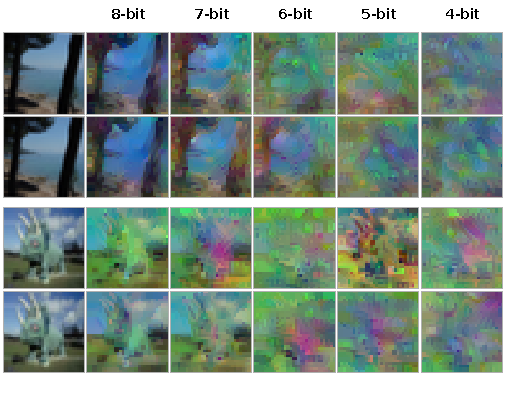
\includegraphics[width=\columnwidth]{paper_assets/quantization_cifar100_imagenet.pdf}%
}{%
  \fbox{\parbox[c][60mm][c]{0.94\columnwidth}{\centering\small
  Figure image not found.\\[2pt]
  Upload \texttt{quantization\_cifar100\_imagenet.pdf}\\
  into \texttt{paper\_assets/} to render it.}}%
}
\caption{Reconstructions at each bit width. Within every block the left column
is naive center decoding and the right the publicly selected \cora{} output,
both at 25,000 inversion iterations; the leftmost column is the private image.
Upper two rows are CIFAR-100 registered indices 11 and 24, lower two ImageNet
indices 0 and 1, all fixed across conditions, with saved Hungarian assignments
reused unchanged. At 4 bits the naive reconstructions flatten while \cora{}
keeps more high-frequency texture --- the behaviour PSNR and SSIM reward and
LPIPS penalizes.}
\label{fig:qualitative}
\end{figure}

\subsection{Sparsification}
\label{sec:sparse}
The first-FC update keeps its largest-magnitude entries at retained fractions
of 50, 30, 20 and 10\%, and naive decoding zero-fills the rest. On CIFAR-100
these runs share the separator, batches and evaluation of the quantization
sweep; the ImageNet study is separate, using the original CPA optimizer with
recovered-source cosine matching. At 50\% retention the discarded entries are
already zero on both datasets: by Eq.~\eqref{eq:mixture} the update inherits
the sparsity of the post-ReLU features, so more than half its coordinates
vanish before any sparsification. The fill radius $\tau$ is then zero, random
filling reduces to zero filling, and the two CIFAR-100 rows coincide exactly,
as they must. Below that level we fill discarded entries uniformly from
$[-\tau,\tau]$ for $\tau$ the smallest retained magnitude. On CIFAR-100,
\cora{} improves LPIPS at 30\% ($0.510$ to $0.489$) and 10\% ($0.570$ to
$0.561$) and loses at 20\%. The ImageNet run at 10\% instead ranks twenty
candidates by an update-consistency score, which replays the known local SGD
with public-model predicted labels, recompresses, and measures the relative
$\ell_2$ distance from the packet; selection is applied twice rather than
fixed at screening. It yields LPIPS $0.630$ against $0.632$ for naive
decoding, better on one metric and worse on two.

\subsection{What the selector finds, and what it misses}
\label{sec:individual}
At 4 bits on ImageNet the first draw, member 00, reached PSNR $11.56$\,dB,
SSIM $0.261$ and LPIPS $0.806$, marginally ahead of the naive control on PSNR
and LPIPS. The selector ranked member 06 first instead, and member 06 is worse
than naive on all three metrics. The margins are small, but the ordering is
not: among the draws whose endpoints we can compare, the ranking did not
return the better one. That row therefore reflects selection at least as much
as sampling, while the corresponding CIFAR-100 row shows the same sampler at
its largest margin of the sweep. Member 00 reached the full budget only
because it ranked third, not as a separately evaluated $K=1$ attack, so this
is an existence observation rather than a measured property of the selector.
We nonetheless report the publicly selected candidate throughout.

\subsection{Budget and scope}
\label{sec:budget}
Randomized search costs $8\times5{,}000+3\times20{,}000=100{,}000$ inversion
iterations per condition, plus 25,000 for the naive control and one separation
per draw and for the center reference. Final per-candidate budgets match while
total search budgets do not, and we make no compute-matched claim: the cosine
schedule is fixed at a 25,000-iteration horizon, so granting the control the
same total would require a different schedule, not a longer run. Every
ImageNet number comes from a single victim batch; CIFAR-100 numbers pool three
independent batches of eight images, which we do not break out here. Several
differences between methods are of the same order as effects we have not
bounded.


\section{Discussion}
\label{sec:discussion}
Degradation with precision needs no appeal to our sampler: naive decoding
degrades too, and the packet carries less about $\U$. What the sampler adds is
spread. Cell width is $s=\|\U\|_\infty/Q_b$, so within a dataset it scales as
$1/Q_b$ and grows by $127/7\approx18$ between 8 and 4 bits. Wider cells cut
both ways, leaving more room for a draw to land nearer $\U$ than the center
and more room for it to land further away, and the ranking decides between
them. On CIFAR-100 the margin is largest at 4 bits, where the cells are
widest; on ImageNet at 4 bits it is negative, yet Section~\ref{sec:individual}
exhibits a draw that came out ahead of the center. That row measures
selection, not sampling. We offer this as the reading most consistent with the
data, not as a mechanism the sweep isolates.

Ranking is limited in a way we can state precisely. The targets in
Eq.~\eqref{eq:score} are estimated from the compressed update itself, so a
candidate can agree with them closely and resemble the private image poorly.
Nor does exact re-encoding establish the stronger property one would want:
that local training on the reconstructed images would reproduce the packet.
The ImageNet sparsification study ranks by exactly that test, but on a
different codec and backend, so these results cannot say which selector is
better. Bounding what ranking costs would require continuing every draw to the
full budget.


\section{Related Work}
\label{sec:related}
Optimization-based gradient inversion reconstructs inputs by matching observed
and synthetic gradients~\cite{zhu2019deep,geiping2020inverting}. CPA instead
treats fully connected gradients as blind source separation solved by ICA,
scaling to larger batches~\cite{kariyappa2023cocktail}, and Zhang et
al.~\cite{zhang2022survey} survey the resulting landscape. On compression as a
defense, Yue et al.~\cite{yue2023gradient} show image information can survive
quantization, sparsification or perturbation; Li et al.~\cite{li2022ggl}
reconstruct under gradient degradation with a GAN prior learned from public
images; and Ding et al.~\cite{ding2024compressed} target sparsified gradients
by compressing synthetic gradients during reconstruction. \cora{} instead
studies randomized decoding and public candidate selection without a
pretrained prior: the sender's quantization is deterministic, and the attacker
samples alternative numerical updates compatible with the observation, ranks
them by feature agreement and total variation, and reports one selected
reconstruction.


\section{Conclusion}
\cora{} reconstructs quantized local updates by sampling compatible decodings
and ranking the resulting candidates with a public feature-based score.
Per-tensor bit sweeps on ImageNet and CIFAR-100 show LPIPS worsening
monotonically from 8 to 4 bits, while PSNR and SSIM recover at low precision
as the reconstructions flatten. Randomized decoding improves LPIPS in eight of
ten conditions; its margin at 4 bits is the largest we measured on one dataset
and negative on the other, where a better draw existed and the ranking did not
return it. The measured curves and reconstructions describe where the
procedure retains image information and where its limitations become
pronounced.


\begin{thebibliography}{9}
\bibitem{zhu2019deep}
L. Zhu, Z. Liu, and S. Han, ``Deep leakage from gradients,'' in \emph{Adv.
Neural Inf. Process. Syst.}, vol. 32, 2019.

\bibitem{geiping2020inverting}
J. Geiping, H. Bauermeister, H. Dr\"oge, and M. Moeller, ``Inverting
gradients---How easy is it to break privacy in federated learning?,'' in
\emph{Adv. Neural Inf. Process. Syst.}, vol. 33, 2020.

\bibitem{kariyappa2023cocktail}
S. Kariyappa, C. Guo, K. Maeng, W. Xiong, G. E. Suh, M. K. Qureshi, and
H.-H. S. Lee, ``Cocktail Party Attack: Breaking aggregation-based privacy in
federated learning using independent component analysis,'' in \emph{Proc.
ICML}, vol. 202, pp. 15884--15899, 2023.

\bibitem{zhang2018lpips}
R. Zhang, P. Isola, A. A. Efros, E. Shechtman, and O. Wang, ``The unreasonable
effectiveness of deep features as a perceptual metric,'' in \emph{Proc. CVPR},
2018.

\bibitem{zhang2022survey}
R. Zhang, S. Guo, J. Wang, X. Xie, and D. Tao, ``A survey on gradient
inversion: Attacks, defenses and future directions,'' in \emph{Proc. IJCAI},
pp. 5678--5685, 2022.

\bibitem{yue2023gradient}
K. Yue, R. Jin, C.-W. Wong, D. Baron, and H. Dai, ``Gradient obfuscation gives
a false sense of security in federated learning,'' in \emph{Proc. USENIX
Security}, pp. 6381--6398, 2023.

\bibitem{li2022ggl}
Z. Li, J. Zhang, L. Liu, and J. Liu, ``Auditing privacy defenses in federated
learning via generative gradient leakage,'' in \emph{Proc. CVPR},
pp. 10132--10142, 2022.

\bibitem{ding2024compressed}
X. Ding, Z. Liu, X. You, X. Li, and A. V. Vasilakos, ``Improved gradient
leakage attack against compressed gradients in federated learning,''
\emph{Neurocomputing}, vol. 608, article 128349, 2024.
\end{thebibliography}

\end{document}
